\documentclass[tikz,border=5pt]{standalone}
\usepackage[T1]{fontenc}
\usepackage{lmodern,amsmath,amssymb}
\usetikzlibrary{arrows.meta,calc,positioning,fit,backgrounds,shapes.geometric,matrix,decorations.pathreplacing,patterns}
\definecolor{ink}{gray}{0.08}
\definecolor{wash}{gray}{0.965}
\definecolor{soft}{gray}{0.45}
\tikzset{box/.style={draw=ink,line width=.65pt,fill=white,align=center,inner sep=4pt,outer sep=0pt,font=\small},flow/.style={draw=ink,line width=.65pt,-{Latex[length=1.8mm,width=1.3mm]},rounded corners=2pt},annotation/.style={font=\scriptsize,text=soft,align=center},groupbox/.style={draw=soft,dashed,line width=.45pt,fill=wash}}
\begin{document}
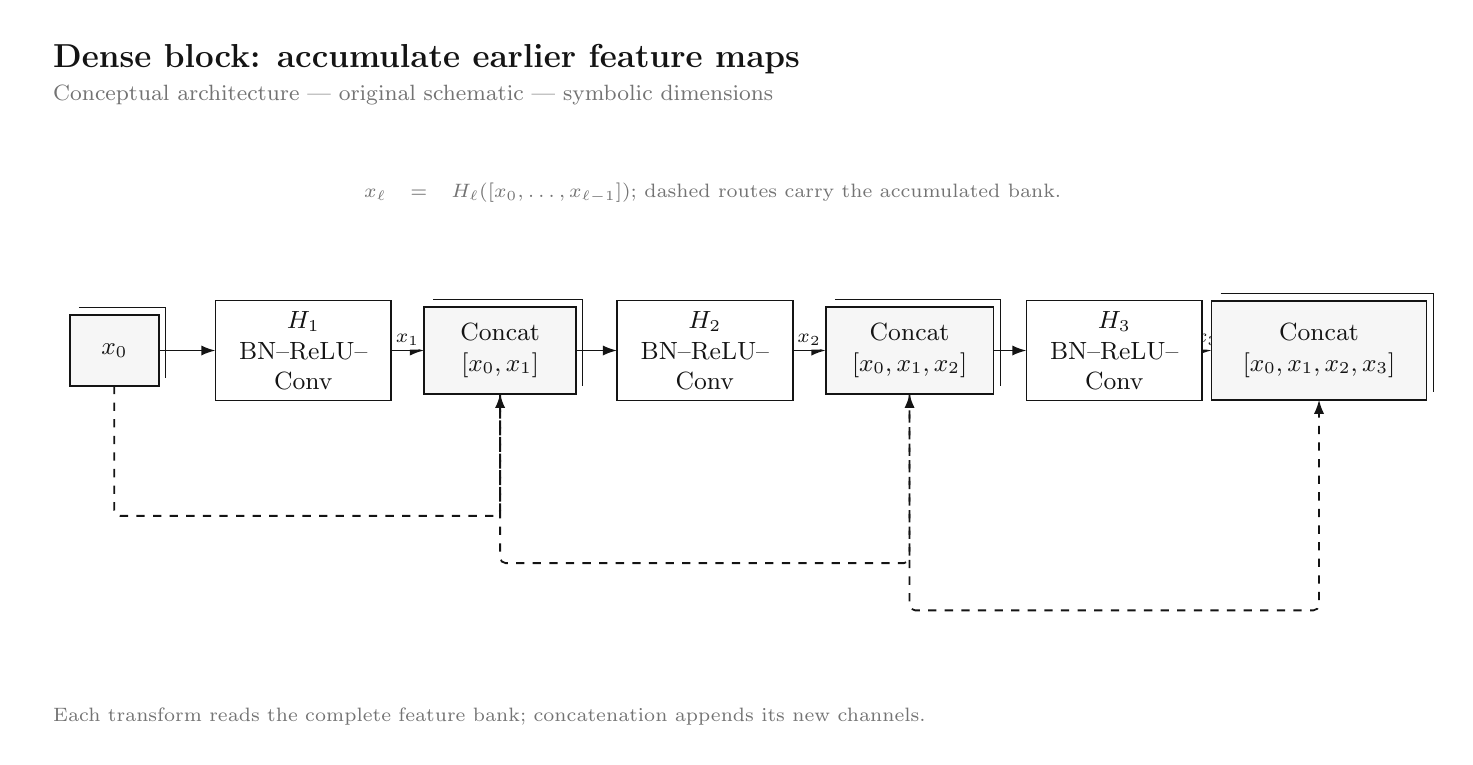
\begin{tikzpicture}[x=1cm,y=-1cm,font=\rmfamily,text=ink]

\path[use as bounding box] (0,0) rectangle (18,9);
\node[anchor=west,font=\large\bfseries] at (.2,.4) {Dense block: accumulate earlier feature maps};
\node[anchor=west,font=\footnotesize,text=soft] at (.2,.85) {Conceptual architecture | original schematic | symbolic dimensions};
\begin{pgfonlayer}{background}
\end{pgfonlayer}
\node[box,fill=wash,minimum width=1.1cm,minimum height=0.9cm,text width=0.8500000000000001cm] (x0) at (1.1,4.1) {$x_0$};
\draw[ink,line width=.4pt] (0.65,3.5499999999999994) -- (1.7500000000000002,3.5499999999999994) -- (1.7500000000000002,4.45);
\node[box,minimum width=2.2cm,minimum height=1.0cm,text width=1.9500000000000002cm] (h1) at (3.5,4.1) {$H_1$\\BN--ReLU--Conv};
\node[box,fill=wash,minimum width=1.9cm,minimum height=1.1cm,text width=1.65cm] (b1) at (6.0,4.1) {Concat\\$[x_0,x_1]$};
\draw[ink,line width=.4pt] (5.1499999999999995,3.4499999999999997) -- (7.05,3.4499999999999997) -- (7.05,4.55);
\node[box,minimum width=2.2cm,minimum height=1.0cm,text width=1.9500000000000002cm] (h2) at (8.6,4.1) {$H_2$\\BN--ReLU--Conv};
\node[box,fill=wash,minimum width=2.1cm,minimum height=1.1cm,text width=1.85cm] (b2) at (11.2,4.1) {Concat\\$[x_0,x_1,x_2]$};
\draw[ink,line width=.4pt] (10.249999999999998,3.4499999999999997) -- (12.35,3.4499999999999997) -- (12.35,4.55);
\node[box,minimum width=2.2cm,minimum height=1.0cm,text width=1.9500000000000002cm] (h3) at (13.8,4.1) {$H_3$\\BN--ReLU--Conv};
\node[box,fill=wash,minimum width=2.7cm,minimum height=1.25cm,text width=2.45cm] (b3) at (16.4,4.1) {Concat\\$[x_0,x_1,x_2,x_3]$};
\draw[ink,line width=.4pt] (15.149999999999999,3.3749999999999996) -- (17.85,3.3749999999999996) -- (17.85,4.625);
\begin{pgfonlayer}{background}
\draw[flow] (x0.east) -- (h1.west);
\draw[flow] (h1.east) -- (b1.west) node[midway,above,fill=white,inner sep=1.5pt,font=\scriptsize] {$x_1$};
\draw[flow] (b1.east) -- (h2.west);
\draw[flow] (h2.east) -- (b2.west) node[midway,above,fill=white,inner sep=1.5pt,font=\scriptsize] {$x_2$};
\draw[flow] (b2.east) -- (h3.west);
\draw[flow] (h3.east) -- (b3.west) node[midway,above,fill=white,inner sep=1.5pt,font=\scriptsize] {$x_3$};
\draw[flow,dashed] (x0.south) -- (1.1,6.2) -- (6,6.2) -- (b1.south);
\draw[flow,dashed] (b1.south) -- (6,6.8) -- (11.2,6.8) -- (b2.south);
\draw[flow,dashed] (b2.south) -- (11.2,7.4) -- (16.4,7.4) -- (b3.south);
\end{pgfonlayer}
\node[annotation,text width=12cm] at (8.7,2.1) {$x_\ell=H_\ell([x_0,\ldots,x_{\ell-1}])$; dashed routes carry the accumulated bank.};
\node[anchor=west,align=left,font=\scriptsize,text=soft,text width=17.6cm] at (.2,8.75) {Each transform reads the complete feature bank; concatenation appends its new channels.};
\end{tikzpicture}
\end{document}
